% =====================================================================
% THIS FILE IS THE SOURCE. Edit it, then rebuild the PDF with:
%     bash tools/compile.sh Unit_03_Building_and_Trusting_a_Model
% (run from the Course_Rewrite folder; it compiles twice and reports
%  page count, overfull boxes, and em dashes)
%
% Do not edit the PDF directly. Figures are the fig_*.pdf files in this
% folder, regenerated by tools/make_module*_slide_figs.py.
%
% Originally converted from the 15-module draft by a one-shot script now
% parked in tools/one_shot_generators/. Re-running those would discard
% anything you change here, so they are kept out of tools/ on purpose.
% =====================================================================
\documentclass[aspectratio=169]{beamer}
\usetheme{default}
\usefonttheme{professionalfonts}
\usepackage{amsmath, amssymb, amsfonts}
\usepackage{graphicx}
\usepackage{booktabs}
\usepackage{bm}
\usepackage{hyperref}

\mode<presentation> {
    \usetheme{Frankfurt}
    \usecolortheme{default}
}

% == notation shortcuts ==
\newcommand{\xbar}{\bar{x}}
\newcommand{\SE}{\mathrm{SE}}
\newcommand{\se}{\widehat{\SE}}

% Recurring motifs (color-coded).
\newenvironment{principle}[1]{\begin{block}{\textbf{Principle:} #1}}{\end{block}}
\newenvironment{trap}[1]{\begin{alertblock}{\textbf{Trap:} #1}}{\end{alertblock}}
\newenvironment{practice}[1]{\begin{exampleblock}{\textbf{In practice:} #1}}{\end{exampleblock}}
\newenvironment{interview}[1]{\begin{exampleblock}{\textbf{You may be asked:} #1}}{\end{exampleblock}}
\newenvironment{yourturn}[1]{%
  \setbeamercolor{block title}{fg=white,bg=orange!80!black}%
  \setbeamercolor{block body}{bg=orange!12}%
  \begin{block}{\textbf{Your turn:} #1}}{\end{block}}
\newenvironment{livedemo}[1]{%
  \setbeamercolor{block title}{fg=white,bg=teal!80!black}%
  \setbeamercolor{block body}{bg=teal!12}%
  \begin{block}{\textbf{Live demo:} #1}}{\end{block}}
\newenvironment{llmcheck}[1]{%
  \setbeamercolor{block title}{fg=white,bg=violet!75!black}%
  \setbeamercolor{block body}{bg=violet!10}%
  \begin{block}{\textbf{LLM check:} #1}}{\end{block}}

\title{Building and Trusting a Model}
\subtitle{Unit 3: From One Predictor to Many, and How Much Flexibility to Allow}
\author{Stat 220 \textbar{} Statistics for Data Science}
\date{}

\begin{document}

\begin{frame}
  \titlepage
\end{frame}

% ======================================================================
\section{Many predictors}
% ======================================================================
\begin{frame}{Where we left off}
\begin{itemize}
  \item Unit 2 fit a line and learned to read a slope, including what happens to it when another
        predictor joins the model.
  \item Now we build models with \emph{many} predictors and confront the question that decides
        whether any of it is real: \textbf{how well does this do on data it has never seen?}
  \item Three days: putting a model together, checking it honestly, and deciding how much
        flexibility the data can actually support.
\end{itemize}
\begin{principle}{the tension, stated plainly}
A model that fits your data perfectly has told you nothing except what your data already said.
\end{principle}
\end{frame}

\begin{frame}{The tension in every model you build}
\begin{itemize}
  \item A model has one real job: do well on data it \textbf{hasn't seen}.
  \item But we only ever fit it on data it \emph{has} seen. So a model can score well for two
        very different reasons: it learned the real signal, or it memorized the noise.
  \item Almost everything in this module is about telling those two apart.
\end{itemize}
\begin{practice}{the shape of this module}
``Your R² jumped from 0.6 to 0.95 when you added more variables. Is it a better model?''
\end{practice}
\end{frame}
\begin{frame}{What this unit gives you}
\begin{columns}[T]
\begin{column}{0.5\textwidth}
\textbf{Things to know}
\begin{itemize}\small
  \item multiple regression, and what ``holding the others fixed'' really means
  \item interactions and transformations
  \item multicollinearity, and what it does to coefficients
  \item overfitting, and why training error is not evidence
  \item cross-validation done correctly, including where leakage sneaks in
  \item regularization and trees: more flexibility, honestly measured
\end{itemize}
\end{column}
\begin{column}{0.5\textwidth}
\textbf{Mistakes to stop making}
\begin{itemize}\small
  \item judging a model by its fit to the training data
  \item chasing $R^2$
  \item preprocessing or selecting features outside the folds
  \item tuning on the test set and then reporting that score
  \item quoting $p$-values from a model built by variable search
  \item reading feature importance as a causal effect
\end{itemize}
\end{column}
\end{columns}
\end{frame}

\begin{frame}{Live experiment: trust, then verify}
\begin{livedemo}{predict shoe size from height}
We need \textbf{10 volunteers} up front.
\begin{itemize}
  \item We can see each person's \textbf{height}, and we record it along with their
        \textbf{shoe size}.
  \item We fit a line that predicts shoe size from height.
  \item Then we will check how good our line is.
\end{itemize}
\end{livedemo}
\vspace{0.2em}
{\tiny\textit{Materials: 10 volunteers, a tape measure if handy. Time: 12 minutes.}}
\vspace{0.2em}
\centering\small
(If a tape measure is handy, height to arm span works even better. Otherwise height to shoe
size needs no tools.)
\end{frame}
\begin{frame}{First, let's ``verify'' on the same 10 people}
\begin{itemize}
  \item We feed each of our 10 volunteers' heights back into the line and compare the predicted
        shoe size to their real one.
  \item The predictions are great. The errors are small. $R^2$ looks high.
  \item So the model is excellent. Are we done?
\end{itemize}
\vspace{0.4em}
\onslide<2->{%
\begin{trap}{that was grading your own homework}
Of course it fits those 10. We \emph{built} the line on them. Checking a model on its own
training data tells you almost nothing about how it will do on someone new.
\end{trap}}
\end{frame}
\begin{frame}{The honest test: people we held out}
\begin{columns}[c]
\begin{column}{0.62\textwidth}
\centering
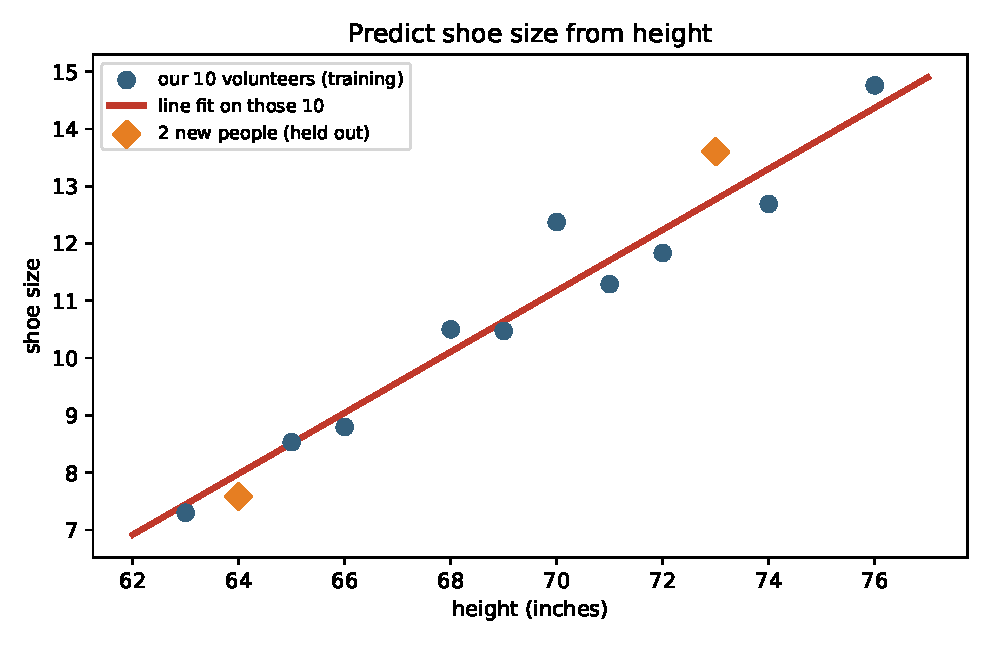
\includegraphics[width=\textwidth]{fig_m3_activity.pdf}
\end{column}
\begin{column}{0.38\textwidth}
\small
Now bring up \textbf{2 new volunteers} (the orange diamonds) who were \emph{not} used to fit
the line. Predict their shoe size, then check.
\vspace{0.4em}

The error on \emph{those} people is the number that counts. That is the whole idea of a
\textbf{train/test split}: fit on some data, judge on data the model never saw.
\end{column}
\end{columns}
\end{frame}
\begin{frame}{From one predictor to many}
\[
   \hat{y} = b_0 + b_1 x_1 + b_2 x_2 + \dots + b_k x_k
\]
\begin{itemize}
  \item Each coefficient is the effect of its predictor \textbf{holding all the others fixed},
        the idea we leaned on for confounding in Part 2.
  \item More predictors can mean a sharper model, or a tangled one where the coefficients fight
        each other. Which one you get depends on how the predictors relate.
\end{itemize}
\begin{principle}{a model is a team of predictors}
The coefficients are not judged one at a time in isolation. Each is reported \emph{given} the
others in the room. Change the lineup and the coefficients change.
\end{principle}
\end{frame}
\begin{frame}{Interactions: when the effect of $x$ depends on something else}
\begin{columns}[c]
\begin{column}{0.56\textwidth}
\centering
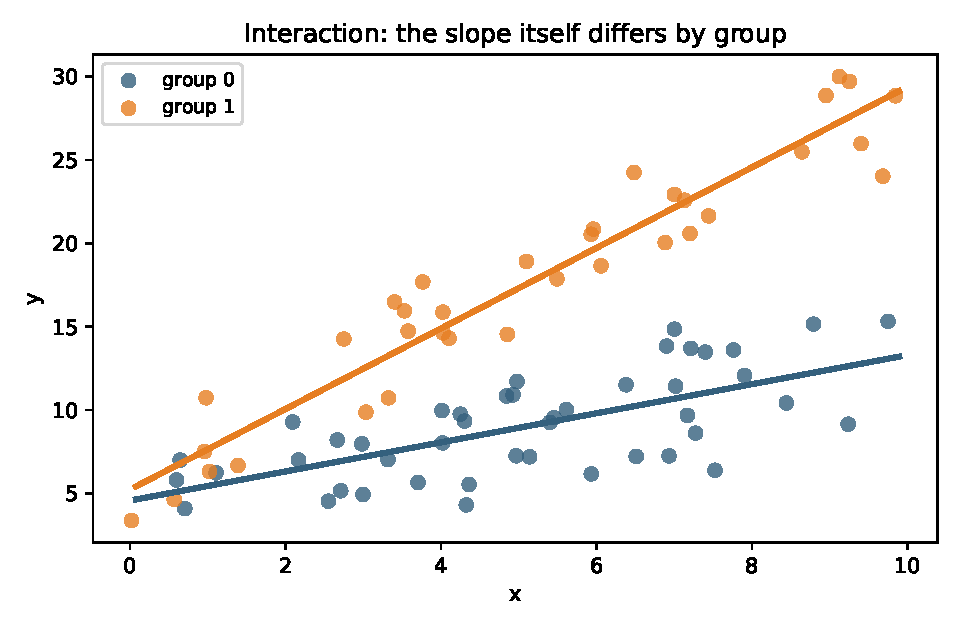
\includegraphics[width=\textwidth]{fig_interaction.pdf}
\end{column}
\begin{column}{0.44\textwidth}
\small
A plain model forces one slope for everyone. An \textbf{interaction} term lets the slope
itself change by group.
\begin{itemize}
  \item ``The effect of price depends on whether it's a weekend.''
  \item Lines are no longer parallel.
\end{itemize}
Add them when you have a real reason to think the effect differs, not just to raise the fit.
\end{column}
\end{columns}
\end{frame}
\begin{frame}{Transformations: when straight lines don't fit}
\begin{columns}[c]
\begin{column}{0.62\textwidth}
\centering
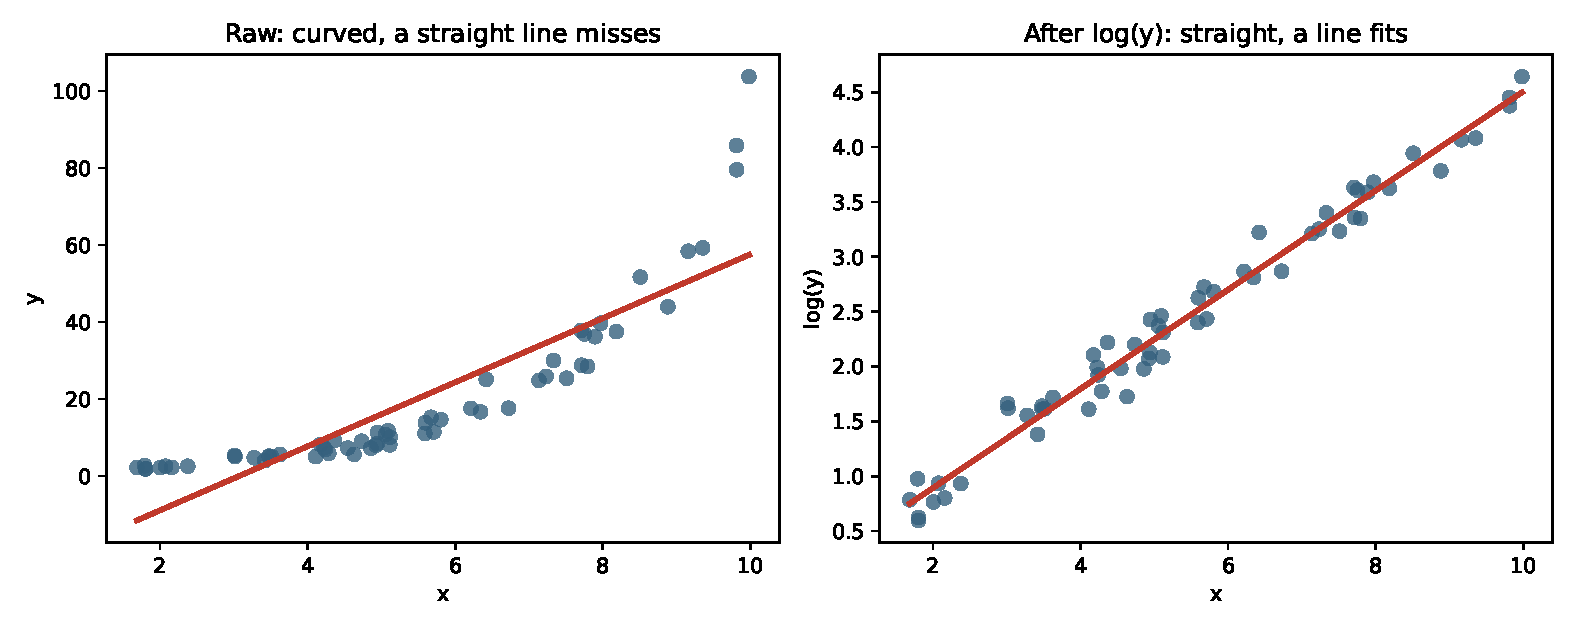
\includegraphics[width=\textwidth]{fig_transform.pdf}
\end{column}
\begin{column}{0.38\textwidth}
\small
Many real relationships curve. A \textbf{log} (or a squared term) can straighten them so a
linear model fits.
\vspace{0.4em}

The cost is interpretation: after a log, a coefficient is read as a \emph{percent} change, not
an absolute one. The model gets simpler and the sentence gets more careful.
\end{column}
\end{columns}
\end{frame}
\begin{frame}{Your turn \#1}
\begin{yourturn}{which model, and why}
You're modeling house price from square footage, and the scatter clearly \textbf{curves
upward}: big houses cost more than a straight line predicts.
\vspace{0.3em}

Turn to a neighbor: would you add a \textbf{squared term}, take a \textbf{log}, or leave it
straight? Practice explaining the trade-off in one sentence.
\end{yourturn}
\end{frame}
\begin{frame}{Your turn \#1: answer}
\begin{itemize}
  \item Either a squared term or a log of price can capture the curve, and both fit better than
        a straight line here.
  \item The trade-off is \textbf{interpretation}: a log lets you say ``each extra 100 sqft is
        about $x\%$ more,'' which is often the cleaner story for prices.
  \item Leaving it straight is the one clearly wrong choice: the model would under-predict big
        houses and over-predict small ones in a systematic way.
\end{itemize}
\begin{principle}{fit the shape, then mind the sentence}
Pick the transformation that matches the shape \emph{and} gives an interpretation you can say
out loud. A better fit you can't explain is rarely worth it.
\end{principle}
\end{frame}
\begin{frame}{Multicollinearity: predictors that say the same thing}
\begin{itemize}
  \item When two predictors are highly correlated (say, square footage and number of rooms),
        the model can't tell which one deserves the credit.
  \item The coefficients become \textbf{unstable}: large standard errors, wide CIs, and signs
        that can flip if you nudge the data.
  \item Prediction is usually fine. It's the \emph{interpretation} of the individual
        coefficients that falls apart.
\end{itemize}
\begin{principle}{shared credit is unstable credit}
Collinear predictors split the credit in an arbitrary way. A big SE on a coefficient is often
the model telling you ``another variable already explains this.''
\end{principle}
\end{frame}
\begin{frame}{How to recognize it, and what it means}
\begin{itemize}
  \item Warning signs: a predictor that ``should'' matter looks insignificant, coefficients
        swing wildly when you add or drop a related variable, or two variables are obviously
        measuring the same thing.
  \item For \textbf{prediction}, you may not care: the team of predictors still forecasts well.
  \item For \textbf{explanation}, you must care: you can't trust either coefficient alone.
\end{itemize}
\begin{trap}{declaring a variable ``unimportant''}
A collinear predictor can look insignificant only because its twin is in the model. Drop the
twin and it springs back to life. Insignificant is not the same as unimportant.
\end{trap}
\end{frame}
% ======================================================================
\section{Honest evaluation}
% ======================================================================
\begin{frame}{Overfitting: learning the noise}
\begin{columns}[c]
\begin{column}{0.56\textwidth}
\centering
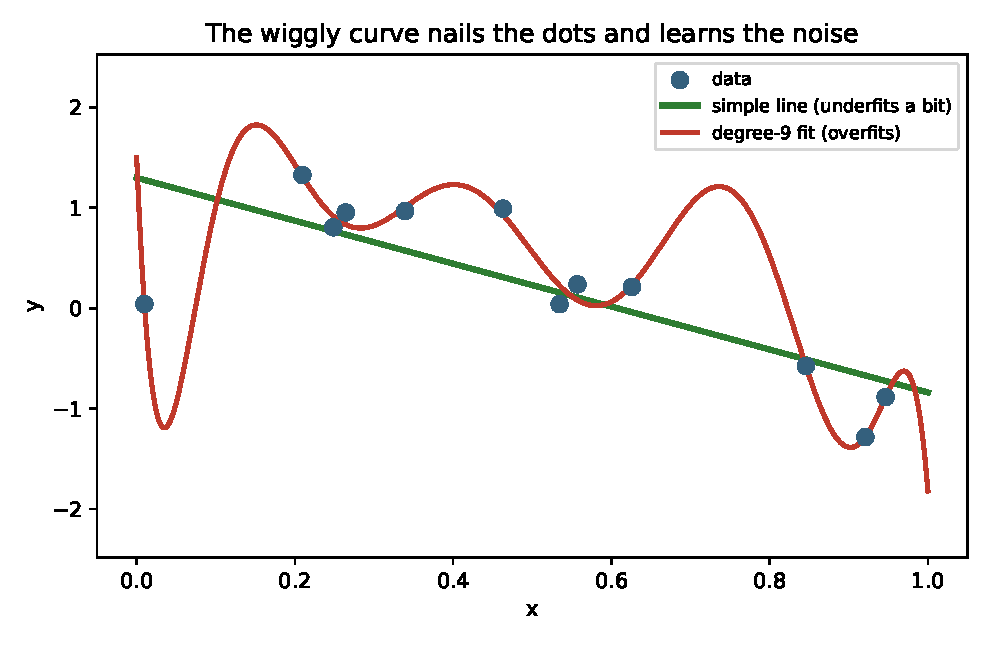
\includegraphics[width=\textwidth]{fig_overfit.pdf}
\end{column}
\begin{column}{0.44\textwidth}
\small
The wiggly curve passes through almost every point. It has the lowest error on this data.
\vspace{0.4em}

But it has learned the \textbf{noise}, the random wobble that won't repeat. On new data it will
do worse than the boring straight line.
\end{column}
\end{columns}
\end{frame}
\begin{frame}{Why $R^2$ alone will mislead you}
\begin{itemize}
  \item Adding any predictor, even pure random noise, can only make in-sample $R^2$ go
        \textbf{up} or stay the same. It never goes down.
  \item So ``$R^2$ improved'' is not evidence of a better model. It's almost guaranteed.
  \item The honest questions are: how does it do on \emph{new} data, and is the gain worth the
        extra complexity?
\end{itemize}
\begin{trap}{the $R^2$ chase}
Judging a model by training $R^2$ rewards complexity for its own sake. It's the single most
common way people fool themselves with a model.
\end{trap}
\end{frame}
\begin{frame}{Training error vs new-data error}
\begin{columns}[c]
\begin{column}{0.6\textwidth}
\centering
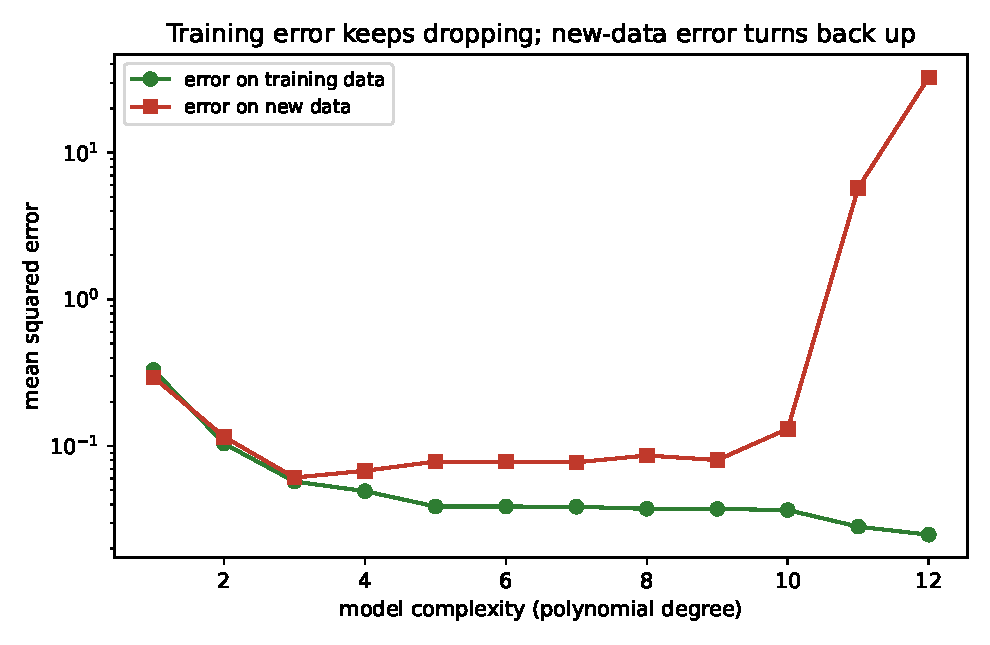
\includegraphics[width=\textwidth]{fig_traintest.pdf}
\end{column}
\begin{column}{0.4\textwidth}
\small
\textbf{Training error} keeps falling as the model gets more complex.
\vspace{0.3em}

\textbf{New-data error} falls, bottoms out, then climbs as the model starts memorizing noise.
\vspace{0.3em}

The best model is near the bottom of the new-data curve, not the bottom of the training curve.
This is why we held people out in the activity.
\end{column}
\end{columns}
\end{frame}
\begin{frame}{The complexity curve, on real data}
\begin{columns}[c]
\begin{column}{0.58\textwidth}
\centering
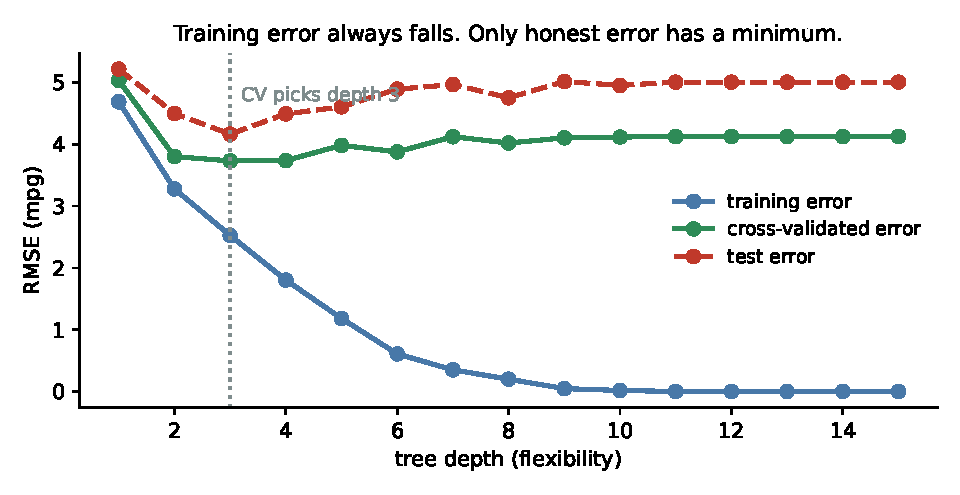
\includegraphics[width=\textwidth]{fig_m11_complexity.pdf}
\end{column}
\begin{column}{0.42\textwidth}
\small
120 training cars, the 6 real predictors plus \textbf{20 columns of pure noise}, which is the
normal condition of a wide dataset.
\begin{itemize}
  \item Training error goes to zero. The model is perfect on the data it saw.
  \item Honest error bottoms out at depth 3 and then gets steadily worse.
\end{itemize}
\end{column}
\end{columns}
\onslide<2->{\centering\small
The deepest tree is 20\% worse than the shallow one, while looking flawless in training.}
\end{frame}
\begin{frame}{K-fold cross-validation}
\begin{enumerate}
  \item Split the data into $K$ parts (5 or 10 is standard).
  \item Train on $K-1$ of them, measure error on the one you held out.
  \item Rotate through all $K$, and average the errors.
\end{enumerate}
\begin{itemize}
  \item Every observation is used for training and, exactly once, for evaluation.
  \item The result estimates how the \emph{procedure} performs on new data, which is what you
        actually want to know.
\end{itemize}
\begin{principle}{cross-validation evaluates a recipe, not a model}
It tells you how well ``fit a depth-3 tree to data like this'' works. That is why you refit on all
the data once the recipe is chosen.
\end{principle}
\end{frame}
\begin{frame}{Doing cross-validation wrong}
The most common and most damaging error in applied machine learning:
\begin{itemize}
  \item Standardizing, imputing missing values, or selecting features using \textbf{the whole
        dataset}, and only then splitting into folds.
  \item Every one of those steps has now seen the held-out data. The reported error is optimistic,
        sometimes wildly so.
  \item The fix: every preprocessing step goes \emph{inside} the fold, applied using only the
        training portion. This is what a pipeline object is for.
\end{itemize}
\begin{trap}{leakage through the back door}
Choosing your 20 best features by correlation with the outcome, and then cross-validating the
model on those 20 features, is not cross-validation. The selection already used the answers.
\end{trap}
\end{frame}
\begin{frame}{The one-standard-error rule}
\begin{itemize}
  \item Cross-validated errors are themselves estimates, with standard errors.
  \item If a depth-3 tree and a depth-7 tree are within one standard error of each other, they are
        not distinguishable, and you should take the \textbf{simpler} one.
  \item Simpler models are more stable over time, easier to explain, cheaper to maintain, and less
        likely to break under distribution shift.
\end{itemize}
\begin{practice}{a strong thing to say}
``The two models were within noise of each other on cross-validation, so I shipped the simpler one
and spent the time on data quality instead.''
\end{practice}
\end{frame}
\begin{frame}{Your turn \#2}
\begin{yourturn}{find the leak}
A teammate reports 94\% cross-validated accuracy on a churn model. Their pipeline:
\begin{enumerate}
  \item Fill missing values with the column mean, computed over all rows.
  \item Keep the 30 features most correlated with churn.
  \item Run 5-fold cross-validation on the resulting dataset.
\end{enumerate}
With a neighbor: what is wrong, and is the true accuracy higher or lower than 94\%?
\end{yourturn}
\end{frame}
\begin{frame}{Your turn \#2: answer}
\begin{itemize}
  \item Steps 1 and 2 both used the \emph{entire} dataset, including every fold's held-out rows.
        The feature selection is the serious one: it looked at the outcome.
  \item The true accuracy is \textbf{lower}, and with many candidate features it can be far lower.
  \item Correct order: split first, then impute using training-fold means, then select features
        using only the training fold, then evaluate.
\end{itemize}
\begin{principle}{the rule that prevents most leakage}
Anything that looks at the outcome, or at all the rows at once, must happen inside the fold.
\end{principle}
\end{frame}
\begin{frame}{Scenario: the R² jumped to 0.95}
\textbf{Setup.} A teammate adds 40 features, and training $R^2$ rises from 0.62 to 0.95 and they
want to ship it.
\begin{itemize}
  \item In-sample $R^2$ almost always rises with more features, so 0.95 on its own is no
        evidence at all.
  \item The test is out-of-sample: split the data, or cross-validate, and compare error on data
        the models never saw.
\end{itemize}
\begin{interview}{how to answer}
``$R^2$ on the training data only ever goes up, so that jump is expected, not impressive. I'd
hold out a test set and compare new-data error. If the 40-feature model isn't better there,
it's just overfitting.''
\end{interview}
\end{frame}
% ======================================================================
\section{Flexibility}
% ======================================================================
\begin{frame}{Live experiment: the class builds a tree}
\begin{livedemo}{you build the tree, one split at a time}
On the board: 30 cars with weight, horsepower, model year, and mpg. The goal is to predict mpg.
\begin{enumerate}
  \item By vote, pick \textbf{one variable and one cutoff} to split the 30 cars into two groups.
  \item I compute the error after your split on those 30 cars, and also on \textbf{10 cars you
        have not seen}.
  \item Keep going. Each round, vote on which group to split next.
\end{enumerate}
\end{livedemo}
\vspace{0.2em}
{\tiny\textit{Materials: the board. Time: 15 minutes.}}
\centering\small We stop when somebody in the room says stop. Then we look at the two error curves.
\end{frame}

\begin{frame}{What happens every time we run it}
\begin{itemize}
  \item The error on the 30 cars falls after \emph{every single split}. It has to: more groups
        means a closer fit to the points being fitted.
  \item The error on the 10 held-out cars falls for the first few splits, flattens, and then
        climbs.
  \item Nobody in the room can feel where that turn happens, and the training error gives no
        warning at all.
\end{itemize}
\begin{principle}{why the stopping rule cannot come from the training data}
You cannot detect overfitting from the data you fit. That is the entire job of the held-out set,
and of the cross-validation we set up earlier.
\end{principle}
\end{frame}

\begin{frame}{What a tree does}
\begin{itemize}
  \item Repeatedly split the data on one variable at a time, choosing the split that most reduces
        error within the resulting groups.
  \item Predict the average outcome (or the majority class) inside each final group.
  \item The result is a \textbf{step function}: no equation, no coefficients, just a sequence of
        yes/no questions.
\end{itemize}
\begin{principle}{trees are good at what lines are bad at}
Interactions and sharp thresholds come free, because every split happens inside the region carved
out by earlier splits. Smooth trends, on the other hand, take a tree many clumsy steps.
\end{principle}
\end{frame}
\begin{frame}{Three fits to the same 392 cars}
\begin{center}
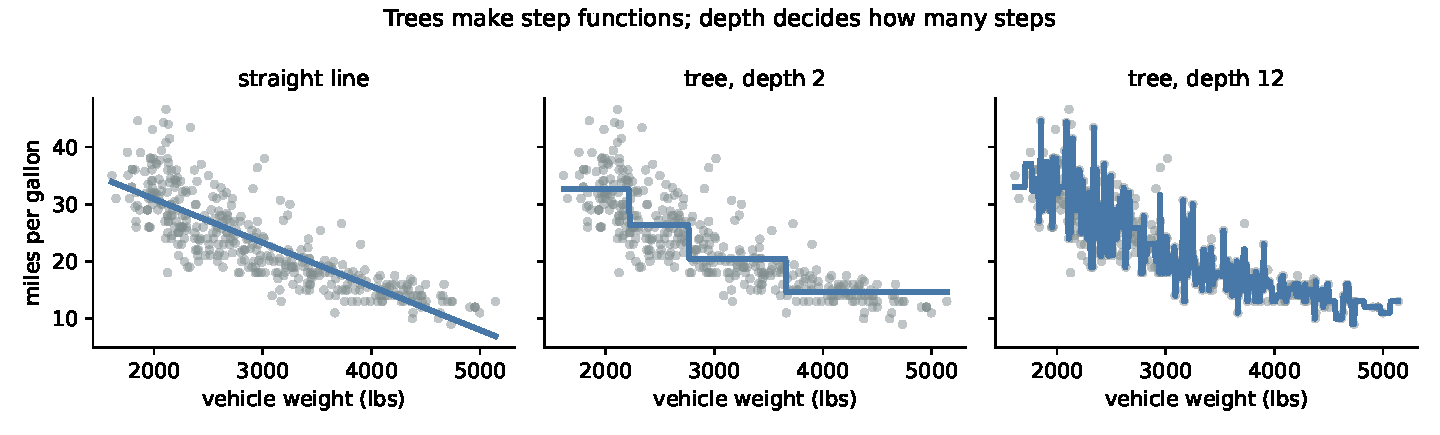
\includegraphics[width=0.95\textwidth]{fig_m11_treefit.pdf}
\end{center}
\vspace{-0.4em}
\small
A line imposes a shape the data does not quite have. A depth-2 tree captures the big picture with
four steps. A depth-12 tree traces individual cars, which is not a discovery about fuel economy.
\end{frame}
\begin{frame}{Searching for variables is a form of overfitting}
\begin{center}
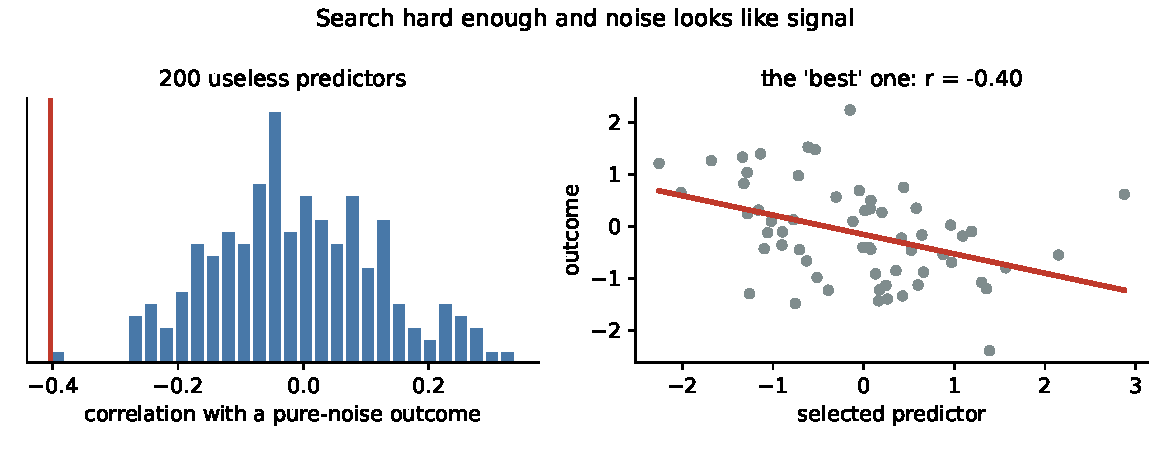
\includegraphics[width=0.9\textwidth]{fig_m11_selection.pdf}
\end{center}
\vspace{-0.4em}
\small
200 predictors, 60 observations, and an outcome that is \emph{pure noise}. The best of the 200
correlates at $0.40$ with the outcome and would be significant at $p < 0.01$ if you reported it
without mentioning the search.
\end{frame}
\begin{frame}{What that means for stepwise selection}
\begin{itemize}
  \item Automated forward/backward selection by $p$-value or AIC picks the winners of many
        comparisons, so the surviving coefficients are biased away from zero.
  \item The printed $p$-values and confidence intervals are then \textbf{invalid}, because they
        assume the model was chosen before the data was seen.
  \item Symptom: an impressive stepwise model that falls apart on next quarter's data.
\end{itemize}
\begin{trap}{significance after selection}
If the variables were chosen by looking at the data, do not report their $p$-values as if they
were. Report out-of-sample performance instead, or validate on fresh data.
\end{trap}
\end{frame}
\begin{frame}{Regularization: shrink instead of choose}
\begin{itemize}
  \item Instead of keeping or dropping variables, penalize large coefficients and let the fit
        balance accuracy against size.
  \item \textbf{Ridge} shrinks all coefficients toward zero, which is ideal when many predictors
        each matter a little and are correlated.
  \item \textbf{Lasso} shrinks and sets some exactly to zero, producing a sparse, readable model.
  \item The penalty strength is chosen by cross-validation, not by taste.
\end{itemize}
\begin{principle}{this is the bias-variance trade you already know}
Regularization is the shrinkage from the estimation module, applied to a whole vector of
coefficients. A little bias, a lot less variance.
\end{principle}
\end{frame}
\begin{frame}{The lasso path, on the cars data}
\begin{columns}[c]
\begin{column}{0.58\textwidth}
\centering
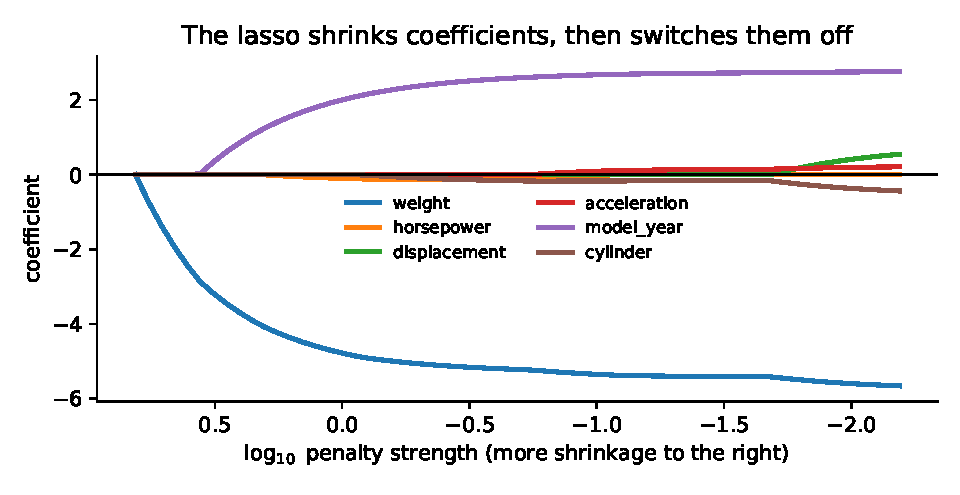
\includegraphics[width=\textwidth]{fig_m11_lasso.pdf}
\end{column}
\begin{column}{0.42\textwidth}
\small
Reading right to left, the penalty weakens and predictors enter the model one by one.
\begin{itemize}
  \item The order of entry is a rough ranking of usefulness.
  \item Correlated predictors (weight and displacement) trade places: the lasso picks one and
        suppresses the other.
\end{itemize}
\end{column}
\end{columns}
\onslide<2->{\centering\small
That last point is a warning: ``the lasso dropped it'' does not mean ``it does not matter.''}
\end{frame}
\begin{frame}{Why one tree is rarely enough}
\begin{itemize}
  \item A single deep tree is \textbf{unstable}: change a few rows and the top split can change,
        rewriting the whole tree.
  \item \textbf{Random forests} average many trees, each fit to a resample of the data and a random
        subset of features. Averaging kills the variance, exactly as in the pooling picture from
        the expectation module.
  \item \textbf{Boosting} instead fits trees in sequence, each one correcting the previous errors.
        It is usually the strongest option on tabular data, and the easiest to overfit.
\end{itemize}
\begin{principle}{ensembles trade explanation for accuracy}
You give up the single readable set of rules and get a model that predicts better and can no
longer be printed on a slide.
\end{principle}
\end{frame}
\begin{frame}{Feature importance is not an effect}
\begin{columns}[c]
\begin{column}{0.58\textwidth}
\centering
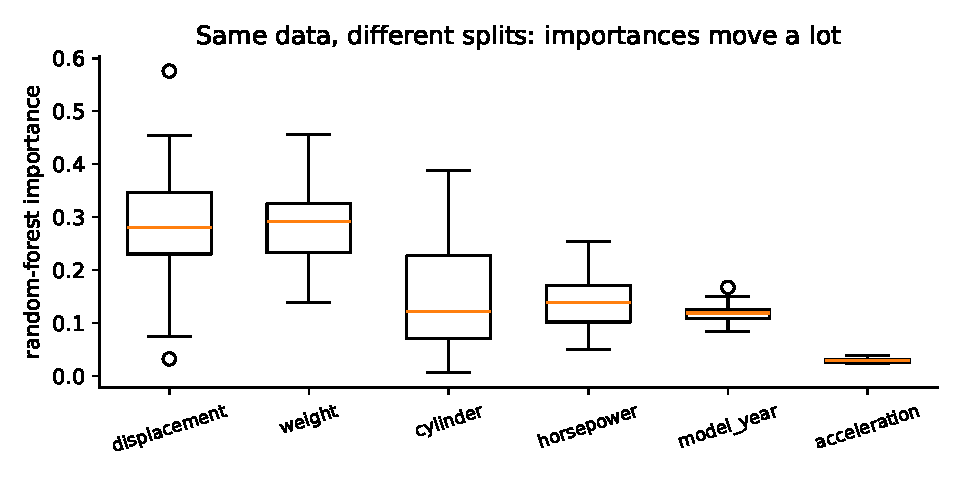
\includegraphics[width=\textwidth]{fig_m11_importance.pdf}
\end{column}
\begin{column}{0.42\textwidth}
\small
Thirty random forests on thirty random splits of the same cars.
\begin{itemize}
  \item The importance of a given predictor swings substantially from run to run.
  \item Correlated predictors split the credit arbitrarily between them.
\end{itemize}
Importance means ``this column was useful for splitting,'' not ``changing this would change the
outcome.''
\end{column}
\end{columns}
\end{frame}
\begin{frame}{Your turn \#3}
\begin{yourturn}{which model do you ship?}
Two models for predicting customer churn:
\begin{itemize}
  \item Logistic regression: cross-validated AUC $0.79 \pm 0.02$, six coefficients you can read.
  \item Gradient boosting: cross-validated AUC $0.81 \pm 0.02$, 400 trees.
\end{itemize}
With a neighbor: which do you ship, and what would change your answer?
\end{yourturn}
\end{frame}
\begin{frame}{Your turn \#3: answer}
\begin{itemize}
  \item The two are within a standard error of each other, so ``more accurate'' is not established.
  \item Ship the \textbf{logistic model} if the output must be explained to customers or
        regulators, if the team maintaining it is small, or if you want to reason about why
        predictions change.
  \item Ship the \textbf{boosted model} if the decision is fully automated, the gain is real at
        scale (one AUC point on ten million decisions is money), and you have monitoring in place.
\end{itemize}
\begin{principle}{accuracy is one input to the decision, not the decision}
The deployment context, not the leaderboard, chooses the model.
\end{principle}
\end{frame}
\begin{frame}{Predict vs.\ explain: pick one on purpose}
\begin{columns}[T]
\begin{column}{0.5\textwidth}
\textbf{Predicting}
\begin{itemize}
  \item You want accurate $\hat{y}$ for new cases.
  \item You don't need clean coefficients.
  \item Judge it by out-of-sample error.
\end{itemize}
\end{column}
\begin{column}{0.5\textwidth}
\textbf{Explaining}
\begin{itemize}
  \item You want to understand one effect.
  \item Coefficients must be trustworthy.
  \item Worry about confounders and collinearity.
\end{itemize}
\end{column}
\end{columns}
\vspace{0.5em}
\begin{principle}{the goal decides the model}
A great prediction model can have meaningless coefficients, and a clean explanatory model can
predict poorly. Decide which you need \emph{before} you build, because it changes every choice.
\end{principle}
\end{frame}
% ======================================================================
\section{LLM check}
% ======================================================================
\begin{frame}{LLM check: mistake or not? (1 of 2)}
\begin{llmcheck}{we asked an LLM to validate a model}
\textbf{We told it:} ``I tried 40 model configurations, picked the one with the best test-set
accuracy (91\%), and want to report that number. Is that fine?''\\[4pt]
\textbf{It answered:} ``Yes, that is standard practice. Since you evaluated on a held-out test set
rather than the training data, 91\% is an unbiased estimate of future performance.''
\end{llmcheck}
\vspace{0.2em}
\centering\small Mistake, or no mistake?
\onslide<2->{%
\begin{trap}{verdict: mistake}
Choosing the best of 40 configurations \emph{by test-set score} makes the test set part of the
training process. 91\% is the maximum of 40 noisy numbers, so it is biased upward. You need a
third split, or nested cross-validation, and you report the score from data used exactly once.
\end{trap}}
\end{frame}
\begin{frame}{LLM check: mistake or not? (2 of 2)}
\begin{llmcheck}{same idea, a different answer}
\textbf{We told it:} ``Two of my predictors are highly correlated, and both have huge standard
errors and look insignificant, yet the model predicts well. What's happening?''\\[4pt]
\textbf{It answered:} ``That's classic multicollinearity: the two carry overlapping
information, so their individual coefficients are unstable with large SEs, even though joint
prediction is fine. Decide whether you really need both.''
\end{llmcheck}
\vspace{0.2em}
\centering\small Mistake, or no mistake?
\onslide<2->{%
\begin{principle}{verdict: no mistake}
This is a correct, careful answer. It separates unstable \emph{coefficients} from fine
\emph{prediction}, which is exactly the right distinction.
\end{principle}}
\end{frame}
% ======================================================================
\section{Consolidate}
% ======================================================================
\begin{frame}{The arc of a modeling project}
\begin{enumerate}
  \item \textbf{Split first.} Hold out a test set and do not touch it again until the end.
  \item \textbf{Start with the simple model.} It is your benchmark, and often your answer.
  \item \textbf{Build the whole pipeline inside the folds}, preprocessing included.
  \item \textbf{Tune complexity by cross-validation}, and apply the one-standard-error rule.
  \item \textbf{Compare candidates on the same folds}, not on separately quoted numbers.
  \item \textbf{Touch the test set once}, to report a final number.
  \item \textbf{Explain what the model uses}, and say plainly that importance is not causation.
\end{enumerate}
\end{frame}
\begin{frame}{Building a model you can defend}
\small
\begin{enumerate}
  \item \textbf{Split first.} Hold out a test set and do not touch it again until the end.
  \item \textbf{Fit the simple model} as your benchmark, and always compare against predicting the mean.
  \item \textbf{Put every preprocessing step inside a pipeline} so it is refit within each fold.
  \item \textbf{Cross-validate:} \texttt{cross\_val\_score(pipe, X, y, cv=KFold(5, shuffle=True))}.
  \item \textbf{Tune complexity on the CV curve}, and take the simplest model within one standard error of the best.
  \item \textbf{Compare candidates on the same folds}, and look at the fold-to-fold spread before declaring a winner.
  \item \textbf{Touch the test set once} and report that number.
\end{enumerate}
\end{frame}

\begin{frame}{The traps, all in one place}
\begin{trap}{the ones that bite most often}
\begin{itemize}
  \item Judging a model on training error, or on $R^2$ alone.
  \item Preprocessing, imputing, or selecting features outside the folds.
  \item Choosing among many models by test-set score and then reporting that score.
  \item Quoting $p$-values from a model whose variables were chosen by search.
  \item Reading feature importance as a causal effect.
  \item Preferring the complex model when the simple one is within noise of it.
  \item Interpreting individual coefficients of two nearly identical predictors.
\end{itemize}
\end{trap}
\end{frame}

\begin{frame}{Ten questions to be able to answer}
\begin{enumerate}\small
  \item How do you know you are not overfitting?
  \item Your $R^2$ jumped when you added 20 features. Better model?
  \item What does $k$-fold cross-validation estimate, and what does it not?
  \item Give three ways leakage sneaks into a cross-validation.
  \item Two predictors are correlated. What happens to their coefficients?
  \item What does the lasso do that dropping variables by $p$-value does not?
  \item Why are $p$-values invalid after stepwise selection?
  \item Your forest beats your regression by 0.02 AUC. Which do you ship?
  \item What does a random forest's feature importance actually measure?
  \item Predict or explain: how does the answer change what you build?
\end{enumerate}
\end{frame}

\begin{frame}{Mastery checklist}
You have this unit when you can, from memory:
\begin{itemize}
  \item interpret a coefficient in a multiple regression, with the right caveat attached
  \item explain interactions and transformations, and when each is called for
  \item recognize multicollinearity and say what it does and does not ruin
  \item draw the training-versus-honest-error curve and explain the gap
  \item run cross-validation correctly, with every preprocessing step inside the fold
  \item apply the one-standard-error rule and defend the simpler model
  \item explain ridge and lasso as shrinkage, and why selection breaks $p$-values
  \item state the limits of feature importance
\end{itemize}
\end{frame}

\begin{frame}{What you should be able to do with software}
\small
Nobody is asking you to memorize syntax. You are expected to know \emph{which} procedure the
question calls for, what to hand it, and what the output means. With an AI assistant open, you
should be able to produce any of these and defend the result.
\begin{center}\footnotesize
\begin{tabular}{p{0.44\textwidth} p{0.46\textwidth}}
\toprule
\textbf{You should be able to} & \textbf{What you would reach for} \\
\midrule
Train/test split & \texttt{train\_test\_split} \\
Cross-validation on the same folds & \texttt{KFold(5, shuffle=True, random\_state=...)} \\
Preprocessing that cannot leak & \texttt{make\_pipeline(StandardScaler(), model)} \\
Ridge and lasso with the penalty chosen for you & \texttt{RidgeCV}, \texttt{LassoCV} \\
A tree, and a forest & \texttt{DecisionTreeRegressor}, \texttt{RandomForestRegressor} \\
Feature importance, with its caveats & \texttt{model.feature\_importances\_} \\
The one-standard-error rule & CV mean plus \texttt{scores.std()/sqrt(k)} \\
\bottomrule
\end{tabular}
\end{center}
\vspace{0.2em}
\centering\small
If you cannot say what the output means, the fact that you produced it is worth nothing.
\end{frame}

\begin{frame}{Where we go next}
\begin{itemize}
  \item We now have models we can trust, judged on data they have never seen.
  \item \textbf{Unit 4} zooms all the way in on a single \textbf{prediction}: when the model
        hands you one number for one case, how wrong is it likely to be, and where does that
        error come from?
\end{itemize}
\begin{principle}{the habit to keep}
Flexibility is not the goal. Honesty about performance is. A simple model you can check beats a
complex one you cannot.
\end{principle}
\end{frame}

\end{document}
